\chapter{Составление схемы замещения сети и определение её параметров}
\label{cha:analysis}

Схема замещения изображенной на рис.~\ref{fig:scheme} электрической сети представляет взаимосвязанную совокупность схем замещения двухцепной воздушной линии (ВЛ) номинального напряжения 110 кВ и трехобмоточных трансформаторов ТДТН-40000/110/35. Сначала следует составить отдельные схемы замещения для каждого элемента электрической сети и рассчитать их параметры

\section{Схема замещения воздушной линии электропередачи}

Воздушные линии электропередачи напряжением 110 кВ допускается представлять П-образной схемой замещения, приведенной на рис.~\ref{fig:pobraz} \cite{веников1998электрические}. В этой схеме поперечные ветви с емкостной проводимостью заменены постоянными реактивными мощностями, равными половине зарядной мощности линии.

\begin{figure}
	\centering
	\includegraphics[width=0.7\textwidth]{inc/svg/zam_vl}
	\caption{П-образная схема замещения ВЛ 110 кВ}
	\label{fig:pobraz}
\end{figure}

Эквивалентное активное сопротивление линии рассчитывается по формуле:

\begin{eqndesc}[H]
	\begin{equation}
		R_\textup{л}=\frac{R_{\text{0}} \cdot L}{n_{\text{ц}}},
		\label{F:req}
	\end{equation}
	
	где $R_{\text{0}}$ "--- удельное активное сопротивление цепи, Ом/км, \\
		$L$ "--- длина линнии, км, \\
		$n_{\text{ц}}$ "--- количество цепей.
\end{eqndesc}

Рассчитаем по формуле \eqref{F:req} активное сопротивление линии ИП-ПС:

\[
R_{\text{ИП-ПС}} = \frac{R_{\text{0}} \cdot L_{\text{ИП-ПС}}}{n_{\text{ц ИП-ПС}}} = \frac{0,204\cdot84}{2} = 8,57\; \text{Ом}
\]

Эквивалентное индуктивное сопротивление линии определяется по формуле:

\begin{eqndesc}[H]
	\begin{equation}
		X_{\text{л}}=\frac{X_{\text{0}} \cdot L}{n_{\text{ц}}},
		\label{F:xeq}
	\end{equation}
	
	где $X_{\text{0}}$ "--- удельное индуктивное сопротивление цепи, Ом/км, определяемое в зависимости от
	среднегеометрического расстояния между проводами фаз линии $D_{\text{сг}}$ и радиуса провода
	$r_{\text{пр}} = \frac{d_{\text{пр}}}{2} = \frac{17,1}{2} = 8,55\; \text{мм}$.
\end{eqndesc}

\[
X_0 = 0,1445\, lg \frac{D_{\text{сг}}}{r_{\text{пр}}} + 0,0157 = 0,1445\, lg \frac{5000}{8,55} + 0,0157 = 0,416\; \frac{\text{Ом}}{\text{км}}
\]

Здесь принято значение усредненного среднегеометрического расстояния $D_{\text{сг}} = 5,0\; \text{м} = 5000\; \text{мм}$ согласно примечанию под таблицей 3.8 \cite{файбисович}.

Рассчитаем по формуле \eqref{F:xeq} индуктивное сопротивление линии ИП-ПС:
\[
X_{\text{ИП-ПС}} = \frac{X_{\text{0}} \cdot L_{\text{ИП-ПС}}}{n_{\text{ц ИП-ПС}}} = \frac{0,416\cdot84}{2} = 17,5\; \text{Ом}
\]

Эквивалентная емкостная проводимость линии:
\begin{eqndesc}[H]
	\begin{equation}
		B_{\text{л}} = n_{\text{ц}} \cdot B_0 \cdot L,
		\label{F:beq}
	\end{equation}

	где $B_0$ "--- удельная емкостная проводимость, См/км, которая так же, как и удельное индуктивное сопротивление, определяется в зависимости от среднегеометрического расстояния между проводами фаз линии $D_{\text{сг}}$ и радиуса провода $r_{\text{пр}}$. 

\end{eqndesc}

\[
B_0 = \frac{7,58\cdot 10^{-6}}{lg \frac{D_{\text{сг}}}{r_{\text{пр}}}} = \frac{7,58\cdot 10^{-6}}{lg \frac{5000}{8,55}} = 2,74\cdot 10^{-6}\; \frac{\text{См}}{\text{км}}
\]

Вычислим по формуле \eqref{F:beq} ёмкостную проводимость линии ИП-ПС:

\[
B_{\text{ИП-ПС}} = n_{\text{ц\, ИП-ПС}} \cdot B_0 \cdot L_{\text{ИП-ПС}} = 2 \cdot 2,74 \cdot 84 = 460,3\cdot 10^{-6}\; \text{См}
\]

Половина зарядной мощности линии 110 кВ:
\begin{eqndesc}[H]
	\begin{equation}
		\frac{Q_{\text{сл}}}{2} = \frac{n_{\text{ц}}\cdot Q_{c0}\cdot L}{2},
		\label{F:Q/2}
	\end{equation}
	где $Q_{c0}$ – удельная зарядная мощность линии, МВар/км.
\end{eqndesc}

Удельная зарядная мощность, соответствующая номинальному напряжению рассматриваемой ВЛ 110 кВ:
\[
Q_{c0} = U_{\text{ном}}^2 \cdot B_0 = 110^2 \cdot 2,74\cdot 10^{-6} = 0,0332\; \frac{\text{МВар}}{\text{км}}
\]

Рассчитаем по формуле \eqref{F:Q/2} половину эквивалентной зарядной мощности двухцепной линии ИП-ПС:
\[
\frac{Q_{c{\text{ИП-ПС}}}}{2} = \frac{n_{\text{ц\, ИП-ПС}}\cdot Q_{c0}\cdot L_{\text{ИП-ПС}}}{2} = \frac{2\cdot 0,0332\cdot 84}{2} = 2,78\; \text{МВар}
\]

Параметры схемы замещения воздушной линии электропередачи определены.

\section{Схема замещения трёхобмоточных трансформаторов}

Составим трехлучевую схему замещения двух параллельно работающих трансформаторов и определим её параметры (см рис. \ref{fig:t_obraz}).

Номинальная мощность трансформатора, номинальные напряжения обмоток, относительное напряжение короткого замыкания лучей, активные потери холостого хода трансформатора и относительное значение тока холостого хода приведены в табл. \ref{tab:tabl4}.

\newpage

\begin{figure}[h]
	\centering
	\includegraphics[width=0.7\textwidth]{inc/svg/t_obraz}
	\caption{Т-образная схема замещения двух параллельно работающих трансформаторов}
	\label{fig:t_obraz}
\end{figure}

\begin{table}[ht]
	\caption{Каталожные данные трансформатора ТДТН-40000/110/35}
	\begin{tabularx}{\textwidth}{|X|X|X|X|X|X|X|X|X|X|}
		\hline
		$S_{\text{т.ном}}$, МВА & \multicolumn{3}{c|}{$U_{\text{ном}}$, обмоток кВ} & \multicolumn{3}{c|}{$U_k$ \%} & $\Delta P_k$, кВт & $\Delta P_\textup{х}$, кВт   & $I_\textup{х}$, \%            \\ \hline
		\multirow{2}{*}{40}   & ВН  & СН   & НН                                   & ВН-СН & ВН-НН & СН-НН         & ВН-СН             & \multirow{2}{*}{43} & \multirow{2}{*}{0,6} \\ \cline{2-8}
		                      & 115 & 38,5 & 11                                   & 10,5  & 17    & 6             & 200               &                     &                      \\ \hline
	\end{tabularx}
	\label{tab:tabl4}
\end{table}

Рассчитаем эквивалентное активное сопротивление лучей высшего, среднего и низшего напряжений схемы замещения для двух трансформаторов:
\begin{eqndesc}[H]
	\begin{equation*}
		\begin{split}
			R_{\text{т.н.экв}} &= R_{\text{т.в.экв}} = R_{\text{т.с.экв}} = \frac{1}{n_{\text{т}}}\cdot \frac{\Delta P_{\text{к.в-с}}}{2}\cdot \frac{U_{\text{ВН}}^2}{S_{\text{т.ном}}^2} = \\
			& = \frac{1}{2}\cdot \frac{200\cdot 10^{-3}}{2}\cdot \frac{115^2}{40^2} = 0,413\; \text{Ом}
		\end{split}
	\end{equation*}

	где $\Delta P_{\text{к.в-с}}$ "--- потери активной мощности, соответствующие опыту короткого замыкания для обмоток высшего и среднего напряжений при разомкнутой обмотке низшего напряжения, МВт; \\
	$S_{\text{т.ном}}$ "--- номинальная мощность трансформатора, МВА; \\
	$U_{\text{ВН}}$ "--- номинальное напряжение обмотки высшего напряжения, кВ; \\
	$n_{\text{т}}$ "--- количество трансформаторов.
	
\end{eqndesc}

Рассчитаем относительные напряжения короткого замыкания обмоток высшего, среднего и низшего напряжений:
\begin{equation*} 
	U_{\text{к.в}} = 0,5\cdot \left(U_{\text{к\, в-с}} + U_{\text{к\, в-н}} - U_{\text{к\, c-н}}\right) =
	0,5 \cdot (10,5+17-6) = 10,8\; \%
\end{equation*}
\begin{equation*} 
	U_{\text{к.с}} = 0,5\cdot \left(U_{\text{к\, в-с}} + U_{\text{к\, с-н}} - U_{\text{к\, в-н}}\right) =
	0,5 \cdot (10,5+6-17) = 0\; \%
\end{equation*}
\begin{equation*} 
	U_{\text{к.н}} = 0,5\cdot \left(U_{\text{к\, с-н}} + U_{\text{к\, в-н}} - U_{\text{к\, в-с}}\right) =
	0,5 \cdot (6+17-10,5) = 6,25\; \%
\end{equation*}

Рассчитаем эквивалентное индуктивное сопротивление высшего, среднего и низшего напряжения лучевой схемы замещения для двух трансформаторов:
\begin{equation*}
	X_{\text{т.в.экв}} = \frac{1}{n_{\text{т}}}\cdot \frac{U_{\text{к.в}}}{100}\cdot \frac{U_{\text{ВН}}^2}{S_{\text{т.ном}}} = \frac{1}{2}\cdot \frac{10,8}{100}\cdot \frac{115^2}{40} = 17,9\; \text{Ом}
\end{equation*}
\begin{equation*}
	X_{\text{т.с.экв}} = \frac{1}{n_{\text{т}}}\cdot \frac{U_{\text{к.с}}}{100}\cdot \frac{U_{\text{ВН}}^2}{S_{\text{т.ном}}} = \frac{1}{2}\cdot \frac{0}{100}\cdot \frac{115^2}{40} = 0\; \text{Ом}
\end{equation*}
\begin{equation*}
	X_{\text{т.н.экв}} = \frac{1}{n_{\text{т}}}\cdot \frac{U_{\text{к.н}}}{100}\cdot \frac{U_{\text{ВН}}^2}{S_{\text{т.ном}}} = \frac{1}{2}\cdot \frac{6,25}{100}\cdot \frac{115^2}{40} = 10,3\; \text{Ом}
\end{equation*}

Рассчитаем эквивалентные потери активной мощности в двух трансформаторах при холостом ходе:
\begin{eqndesc}
	\begin{equation*}
		\Delta P_{\text{x.экв}} = n_{\text{т}}\cdot \Delta P_{\text{х}} = 2\cdot 43 = 86\; \text{кВт},
	\end{equation*}
	где $\Delta P_{\text{х}}$ "--- активные потери холостого хода, кВт.
\end{eqndesc}

Рассчитаем эквивалентные потери реактивной мощности в двух трансформаторах при холостом ходе по формуле:
\begin{eqndesc}
	\begin{equation*}
		\Delta Q_{\text{x.экв}} = n_{\text{т}}\cdot \frac{I_x}{100}\cdot S_{\text{т.ном}} = 2\cdot \frac{0,6}{100}\cdot 40 = 0,48\; \text{МВар}
	\end{equation*}
	где $I_{\text{х}}$ "--- относительное значения тока холостого хода, \%.
\end{eqndesc}

\section{Общая схема замещения сети}

Составим на рис. \ref{fig:obshaya_schema} общую схему замещения сети, состоящую из двух параллельно работающих трансформаторов и линии ВЛ 110 кВ, и укажем на ней все числовые значения рассчитанных параметров и их размерностей.

\begin{sidewaysfigure}
	\centering
	\includegraphics[width=0.9\textwidth]{inc/svg/obshaya_schema}
	\caption{Общая схема замещения двух параллельно работающих трансформаторов и ВЛ}
	\label{fig:obshaya_schema}
\end{sidewaysfigure}
%%% Local Variables:
%%% mode: latex
%%% TeX-master: "rpz"
%%% End:
